Durante este capítulo serão descritas em detalhes as diferentes etapas de funcionamento da luva Hand.io e será explicado como os objetivos deste trabalho serão atingidos.

\section{Visão geral do método da Hand.io}




\todo{Apresentar um descrição da visão geral do método proposto usando a big picture}


%\begin{figure}
%	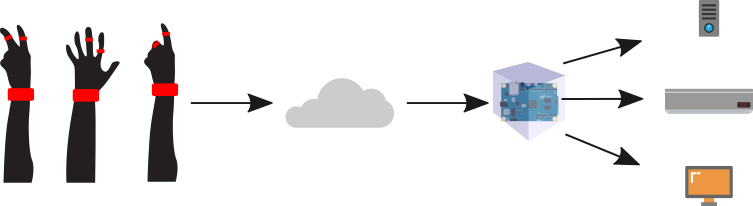
\includegraphics{big_picture}
%\end{figure}






\section{Captura de Dados Baseado em Movimentos de Amplitude de Punho e Mão}

Os gestos realizados pelo usuário serão capturados utilizando um sensor acelerômetro e giroscópio que serão enviados em tempo real até uma central de reconhecimento de padrões que terá seu funcionamento detalhado na seção seguinte. 



\section{Reconhecimento de Padrões Baseado em Movimentos e Ações}



\section{Modelo de Conexão Entre Dispositivos Eletrônicos}

\section{Inferência de Comportamentos para Acionamento de Dispositivos Eletrotônicos}

\section{Modelo de Prototipação}

\begin{figure}
    \centering
    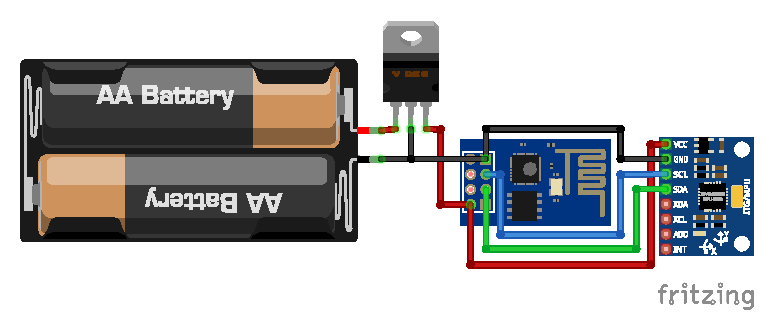
\includegraphics{resources/esquematico_tcc_bb.pdf}
    \caption{Esquemático do protótipo da luva}
    \label{fig:my_label}
\end{figure}

\begin{figure}
    \centering
    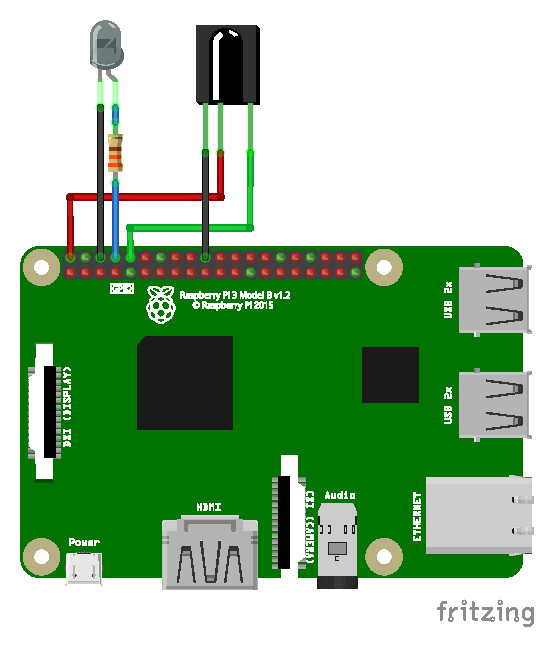
\includegraphics{resources/esquematico_central_bb.pdf}
    \caption{Esquematico da central de processamento de sinais e execução de ações}
    \label{fig:esq_central}
\end{figure}

%\section{Cronograma}